\documentclass[12pt]{article}

\usepackage[cm]{fullpage}
%\setlength{\topmargin}{-0.5in}
\setlength{\oddsidemargin}{-0.25in}
\setlength{\evensidemargin}{-0.25in}
\setlength{\textwidth}{7in}
\setlength{\textheight}{9.5in}

% do not indent outermost itemize environ
\setlength{\leftmargini}{0.5in}

\usepackage{enumitem}
\usepackage{hyperref}
\usepackage{amssymb}
\usepackage{amsmath}
\usepackage{multicol}
\usepackage{array, latexsym}
\usepackage{times}
\usepackage{time}
\usepackage{subfigure}
\usepackage{graphics}
\usepackage{graphicx}
\usepackage{epstopdf}
\usepackage[T1]{fontenc}
\newcommand{\To}{\Rightarrow}
\newcommand{\del}{\nabla}
\newcommand{\R}{\mathbb{R}}
\newcommand{\C}{\mathcal{C}}
\newcommand{\N}{\mathcal{N}}
\newcommand{\A}{\mathcal{A}}
\renewcommand{\O}{\mathcal{O}}
% \renewcommand{\N}{\mathbb{N}}
\newcommand{\ben}{\begin{enumerate}}
\newcommand{\een}{\end{enumerate}}
\newcommand{\eps}{\varepsilon}
\renewcommand{\epsilon}{\varepsilon}
\newcommand{\p}{\partial}
\newcommand{\<}{\langle}
\renewcommand{\>}{\rangle}
\renewcommand{\subset}{\subseteq}
\newcommand{\cont}{\Rightarrow \Leftarrow}
\newcommand{\back}{\backslash}
\newcommand{\norm}[1]{\|{#1}\|}
\newcommand{\abs}[1]{|{#1}|}
\newcommand{\ip}[1]{\langle{#1}\rangle}
\newcommand{\m}[1]{{\mathbf{#1}}}
\newcommand{\sts}{\m{S}^\textrm{T}\m{S}}
\newcommand{\rank}{\textrm{rank}}
\newcommand{\X}{\mathcal{X}}
\newcommand{\Y}{\mathcal{Y}}
\def\ds{\displaystyle}
\def\d{\partial}
%\renewcommand{\arraystretch}{2.5}

%\newcommand{\ModScenTitle}{Disease Modeling Revivisted}
%\newcommand{\extraTitleInfo}{\small{(adapted from \href{http://math.smith.edu/~callahan/cic/book.pdf}{{\it Calculus in Context}, Callahan and Hoffman,} and from a project developed by MacCluer, Bourden and Kriete, the authors of \href{https://bookstore.ams.org/mbk-125?_ga=2.181115879.1531767786.1587142304-462795727.1586992848}{{\it Differential Equations: Techniques, Theory, and Applications}.}})}


\newcommand{\ModScenTitle}{Disease Modeling, Revisited\footnote{These materials are adapted from \href{http://math.smith.edu/~callahan/cic/book.pdf}{{\it Calculus in Context}, Callahan and Hoffman,} and from a project developed by MacCluer, Bourden and Kriete, the authors of \href{https://bookstore.ams.org/mbk-125?_ga=2.181115879.1531767786.1587142304-462795727.1586992848}{{\it Differential Equations: Techniques, Theory, and Applications}.}}}





\begin{document}
\pagestyle{empty}
%Modeling scenario header

\pagestyle{empty}
\noindent\rule{7in}{0.4pt}
\begin{center}
{\sc 
\noindent Differential Equations\\
Modeling Scenario: \ModScenTitle\\
%\extraTitleInfo
}
\end{center}
\noindent\rule{7in}{0.4pt}


\subsection*{Previous Model}

\noindent  Recall our previous for spread of an infectious disease.  We begin by recalling the following
definitions.
	\begin{center}
	\begin{tabular}{|c|l|l|}
	\hline
	variable	& meaning		& units\\
	\hline \hline
	$N$	& \mbox{\hspace{3in}}	& \mbox{\hspace{2in}}\\
	\hline
	$t$	& 					&\\
	\hline
	$I(t)$	&					& \\
	\hline
	$k$	&					& \\
	\hline
	\end{tabular}
	\end{center}

\noindent  We also made some assumptions.
	\begin{itemize}
	\item  The total population size remains constant.  That is, our populations experiences no deaths,
		no births, no emigration and no immigration.
	\item  The disease is spread through contact between susceptible people (i.e., people who have not
		contracted the disease) and those who have contracted the disease.
	\item  People who have the disease remain infectious.  They can continue to spread the disease
		indefinitely.
	\end{itemize}
	
\noindent Based on this, we came up with the following idea for a model:
\begin{quote}{\it the rate of spread of the disease is proportional to the product of (the number of people who are susceptible) and (the number of people who are infected)}
\end{quote}

\noindent  When we translate to a mathematical statement, we have
\vspace{1cm}

\noindent  We were able to solve this DE for the function $I(t)$ using separation of variables, and then 
we plotted the solution and compared with the data we collected in class.  Here's an example of such a plot:
	\begin{center}
	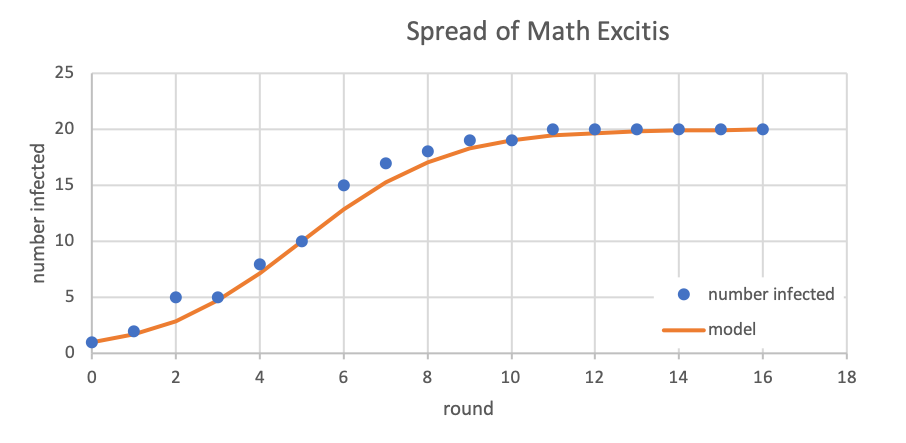
\includegraphics[scale = 0.75, trim = 0 0 0 0]{example_data_and_model_plot.png}
	\end{center}
	
\noindent  This model does a decent job of modeling the data we collected in class for the fictitious
disease Math Excitis, but it would have significant shortcomings if we tried to use for other diseases,
among which are that we assumed:
	\begin{itemize}
	\item  \line(1,0){450}
	\item  \line(1,0){450} 
	\end{itemize}

\noindent  We can overcome some of these shortcomings by considering a more robust model.  We will
begin with another common disease model, the SIR (read S-I-R) model, and we will discuss how to solve it.
Then we will discuss modifications of the model that might make it suitable for studying the COVID-19
pandemic. \\ \vspace{1cm}

%%%%%%%%%%%%%%%%%%%%%%%%%%%%%%%%%%%%%%%%%%%%%%%%%%%%%
\subsection*{Introduction to SIR Disease Modeling}

\noindent  We will eventually discuss modeling the COVID-19 outbreak using data available at this time,
but in order to warm up to the models, let's consider a disease for which we have more information. 
Let's imagine we are modeling a measles outbreak.\\

\noindent  As with all models, we will be making some assumptions as we build our model.
	\begin{itemize}
	\item  The disease is mild, so everyone who falls ill eventually recovers.
	\item  Once someone has contracted the disease and recovers, they have permanent immunity.
	\item  The population size is fixed in size and contained.
	\item  At any time, the population can be split into three distinct classes:
		\begin{itemize}
		\item  {\bf Susceptible:}  those who have never had the disease and may catch it
		\item  {\bf Infected:}  those who currently have the disease and are contagious
		\item  {\bf Recovered:}  those who have already had the disease and are immune from
			catching it again.\\
		\end{itemize}
	\end{itemize}

\noindent  Hopefully you can now see why this model is named the SIR model.  We can visualize
this idea as in the figure below.\\
	\begin{center}
	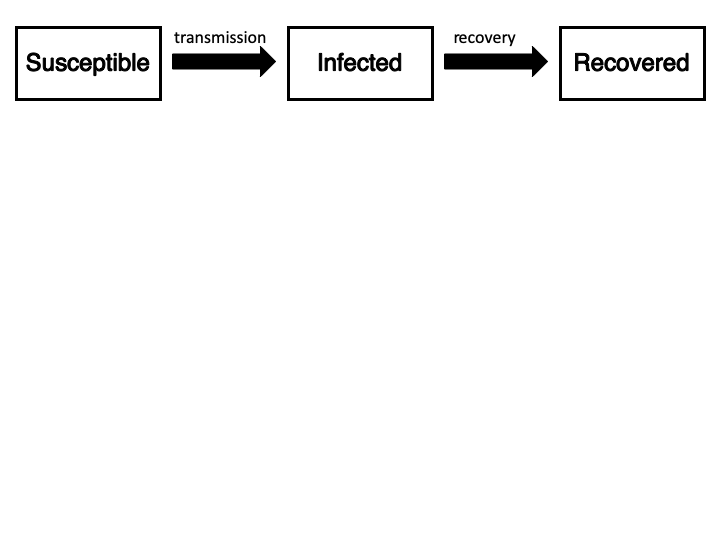
\includegraphics[scale = 0.6, trim = 0 5.5in 0 0]{SIR_flow.png}
	\end{center}
\newpage
\noindent  Notice we again assume that the total population size remains constant.  That means that
only the proportion of people in the carious categories changes, as demonstrated in these pie charts.
	\begin{center}
	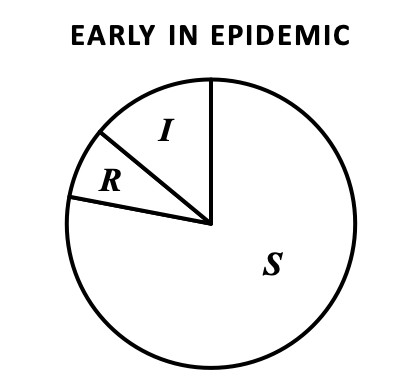
\includegraphics[scale = 0.75, trim = 0 0in 0 0]{pie1_early.png} %\hspace{0.5cm}
	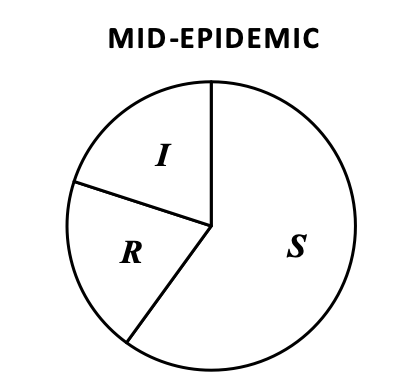
\includegraphics[scale = 0.75, trim = 0 0in 0 0]{pie2_mid.png} %\hspace{0.5cm}
	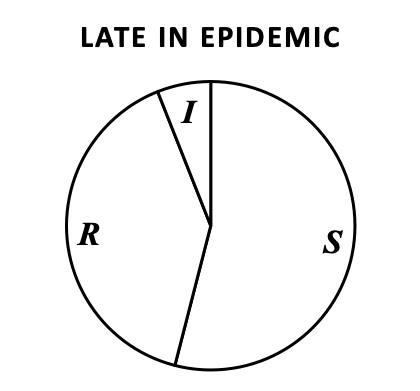
\includegraphics[scale = 0.75, trim = 0 0in 0 0]{pie3_late.png}
	\end{center}
	
\noindent  Notice that we have three classes of people, but the number of people in each class changes
over time.  Our goal would be to determine what happens to each of these numbers over time.  But let's
use our intuition for a moment and think about how we ``expect'' each of the numbers to change over time.
When we say there's an outbreak of measles, we expect the number of cases to increase relatively 
quickly, followed by a gradual decrease.  We might expect to see something like the plot below.
	\begin{center}
	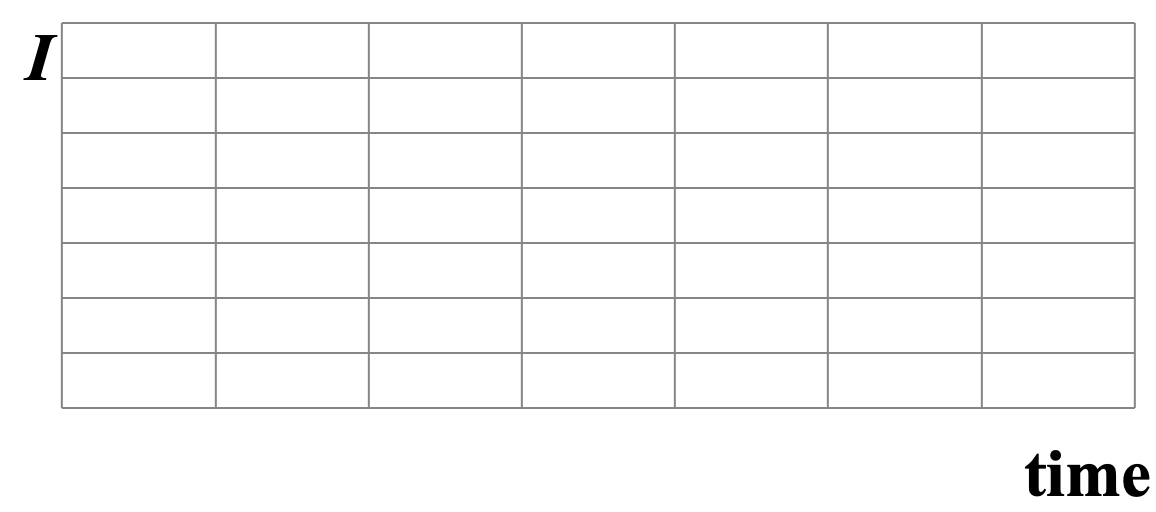
\includegraphics[scale = 0.4]{blank_I_axes.png}	
	\end{center}
	
\noindent  Let's continue down this path by thinking about what the plot of the susceptible population might
look like over time.  We know that the susceptible population continually decreases as people fall ill.  It 
might decrease to zero (if everyone falls ill) or it might decrease to a value above zero.  At the same time, 
we would expect to see a steady increase in the the recovered population, with that population leveling
off eventually.
	\begin{center}
  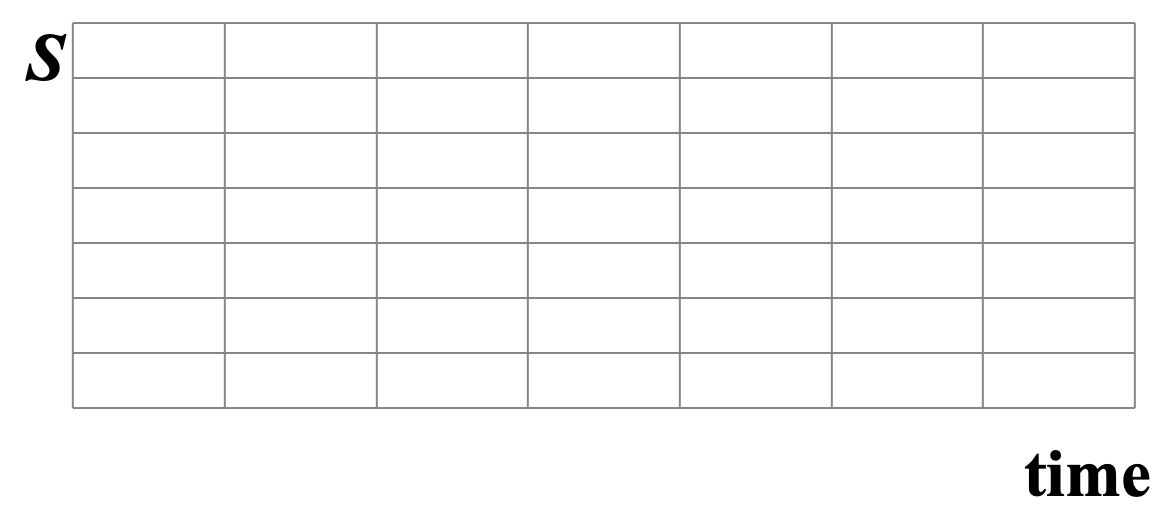
\includegraphics[scale = 0.35]{blank_S_axes.png} \hspace{0.5cm}
	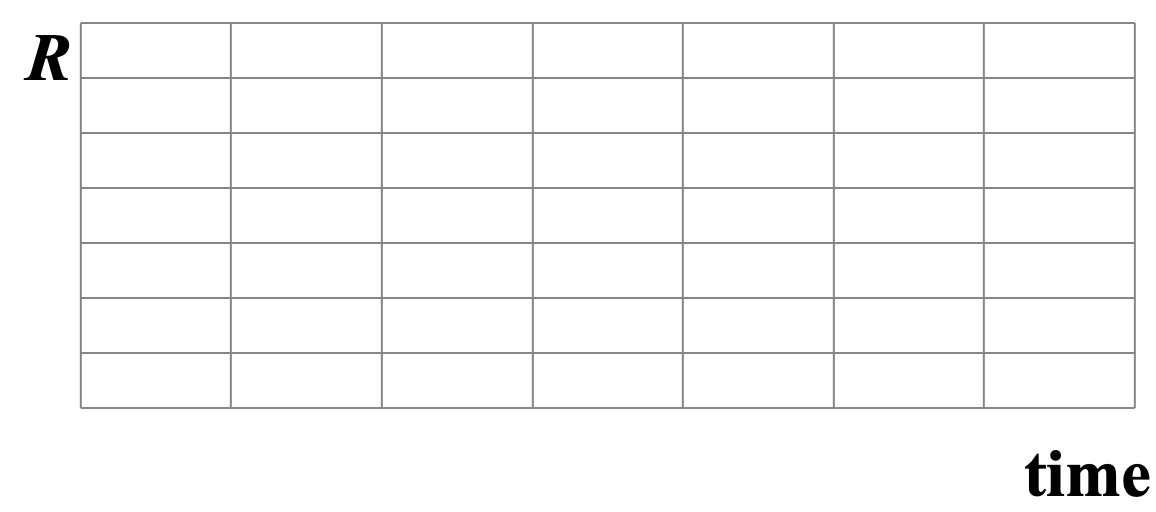
\includegraphics[scale = 0.35]{blank_R_axes.png}
	
	\end{center}
	
\noindent These graphs represent what we think might happen.  They also might lead us to some
questions that would be of interest to someone studying the outbreak.
	\begin{itemize}
	\item  When do we expect the disease to reach its peak?
	\item  How many people do we expect are infected at that time?
	\item  Do we expect everyone will have contracted the disease?  If not, what percentage can we 
		expect will have have contracted the disease?
	\end{itemize}
\newpage
\noindent  As we are now seeing, the answers to these questions may matter a lot in terms of knowing 
whether we have enough resources to care for those with an illness or knowing what preventative
measures we should emplace so that we ``flatten'' the infected curve.  While it's not as critically important
for a measles outbreak as it is for the current COVID-19 pandemic, scientists and healthcare workers 
do want to know this information for every disease circulating because there are always at-risk populations
who may succumb to what we might consider more benign diseases.\\

\noindent  As we discovered in our first model of disease spread, we may not be able to immediately write 
down functions for the curves in those graphs, but we can often describe the 
\line(1,0){75}
of the disease spread and recovery.  In other words, we can write equations for the 
\line(1,0){125}.
Then we would hope to solve those differential equations so we could answer those important questions.\\

%%%%%%%%%%%%%%%%%%%%%%%%%%%%%%%%%%%%%%%%%%%%%%%%%%
\subsection*{Rate of recovery}
\noindent  When someone gets the measles, recovery is usually just a matter of time.  People may be 
infectious for about 8 days\footnote{The \href{https://www.cdc.gov/measles/transmission.html}{Centers 
for Disease Control and Prevention} states that people can spread the measles from about 4 days prior to 
the appearance of a rash through about 4 days after the rash appears.}.  If, on any given day during the
outbreak, we examine the infected population $I$, we would see some that were infected 1 day ago,
some that were infected 2 days, ago, etc., all the way up to those infected 8 days ago.  Those that were 
infected 8 days prior will then transition to the recovered class, $R$.  Without having other information, we
might assume that one-eighth of the infected population would recover today.  That is,
\[ \mbox{the change in the recovered population} = \mbox{\hspace{1.5in}}. \]
	
Note that we are talking about the {\it rate of change of $R$} with respect to time...also known as the
derivative.  That is,
\vspace{2cm}

	
\noindent  Note that the coefficient $\frac{1}{8}$ is specific to the measles.  When we do decide to
apply this model to other diseases, we can generalize this as 
\vspace{2cm}

\noindent where $b$ is a positive constant that we will refer to as the 
\line(1,0){100}.\\

\noindent  We have a differential equation!  We'll examine it more in a bit, but let's set it aside for a moment
and see if we can come up with differential equations for the other two classes.
\newpage
%%%%%%%%%%%%%%%%%%%%%%%%%%%%%%%%%%%%%%%%%%%%%%%%%%
\subsection*{Rate of transmission}
\noindent  We will now focus on how people contract the disease.  We have actually already thought about
this in our initial disease model.  We will use the same logic we did then:
\begin{quote}{\it the rate of spread of the disease is proportional to the product of (the number of people 
who are susceptible) and (the number of people who are infected).}
\end{quote}
\noindent The difference now is that this affects two components of the model.  As people transition from
susceptible to infected, we would see the susceptible population decrease and we would see a 
corresponding increase in the number of infected.  If we focus on the susceptible population for a moment,
we could translate that same sentence as:
\begin{quote}{\it the change in the susceptible population is proportional to the product of (the number of people 
who are susceptible) and (the number of people who are infected).}
\end{quote}
Translating this to a mathematical equation, we have
\vspace{2cm}

\noindent where $a$ is a positive constant that we will refer to as the 
\line(1,0){100}.
Note that the negative 
sign in the differential equation is due to the fact that the susceptible population decreases as people
transition to the infected population through interaction between susceptible people and infected people.\\

%%%%%%%%%%%%%%%%%%%%%%%%%%%%%%%%%%%%%%%%%%%%%%%%%%
\subsection*{The complete model}
\noindent  We need only come up with a differential equation for the infected class, $I$.  We actually
already have all the information we need.  We know that the infected population increases as people
transition from the susceptible population, and it decreases as people transition out to the recovered
population.  Since we have already developed equations for those transitions, we use those to build
the equation for the rate of change in $I$.  Thus, we have the following.
\vspace{7cm}

	
\noindent  Notice that we have three differential equations.  Before we get too far, let's think about the 
independent and dependent variables.  Based on the term derivative terms we can see that $t$ is the 
independent variable while $S$, $I$, and $R$ are dependent variables.  Let's formalize everything we've done so far.

\newpage

%%%%%%%%%%%%%%%%%%%%%%%%%%%%%%%%%%%%%%%%%%%%%%%%%%
\subsection*{The SIR Model}
	\begin{center}
	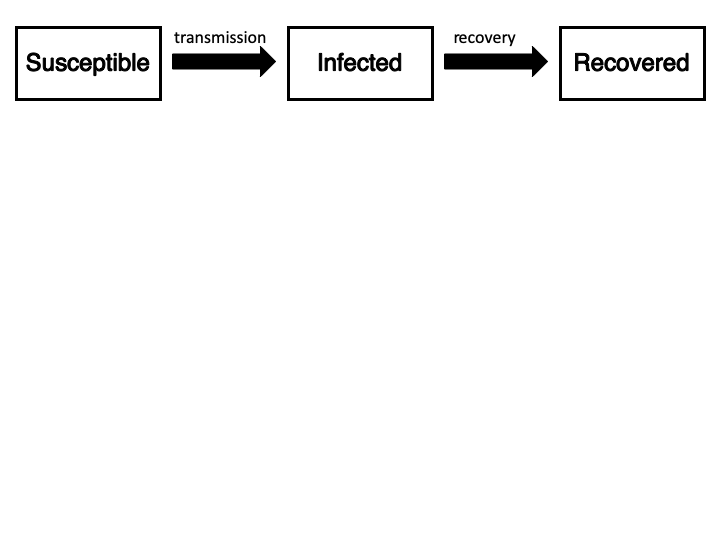
\includegraphics[scale = 0.6, trim = 0 6in 0 0]{SIR_flow.png}
	\end{center}
\noindent  The SIR model is used to model the spread of disease in a population under the following assumptions:
	\begin{itemize}
	\item  The disease is mild, so everyone who falls ill eventually recovers.
	\item  Once someone has contracted the disease and recovers, they have permanent immunity.
	\item  The population size is fixed in size and contained.\\
	\end{itemize}
	
\noindent We define the following variables and constants.
\renewcommand{\arraystretch}{1}
	\begin{center}
	\begin{tabular}{|c|l|l|}
	\hline
	variable/	&					&\\
	constant	& meaning			& units\\
	\hline \hline
	$t$	& time (independent variable)	& days\\
	\hline
	$S$	& the number susceptible at time $t$	& number of people\\
		& (a dependent variable)		&\\
	\hline
	$I$	& the number infected at time $t$	& number of people\\
		& (a dependent variable)		&\\
	\hline
	$R$	& the number recovered at time $t$	& number of people\\
		& (a dependent variable)		&\\
	\hline
	$a$	& transmission coefficient		& days$^{-1} \cdot $people$^{-1}$\\
		& (a constant)				&\\
	\hline
	$b$	& recovery coefficient		& days$^{-1}$\\
		& (a constant)				&\\
	\hline
	\end{tabular}
	\end{center}
\renewcommand{\arraystretch}{1.5}
\noindent The model is given by the following set of three differential equations.
	\begin{align}
	 \frac{dS}{dt}	&= -aSI  \\
	 \frac{dI}{dt}	&= \hspace{0.3cm}aSI - bI	 \\
	 \frac{dR}{dt}	&=  \hspace{1.5cm}bI
	\end{align}
\noindent You may prefer an alternate notation for the exact same set of equations.
	\begin{align}
	S'(t)	&= -a\cdot S(t) \cdot I(t)  					\label{SEqun}\\
	 I'(t)	&= \hspace{0.3cm}a\cdot S(t) \cdot I(t) - b\cdot I(t)		\label{IEqun}\\
	 R'(t)	&=  \hspace{3.1cm}b\cdot I(t)		\label{REqun}
	\end{align}
\noindent  These are mathematically identical, but the second set may help remind you that $S$, $I$,
and $R$ are functions of the independent variable $t$.\\
	
%%%%%%%%%%%%%%%%%%%%%%%%%%%%%%%%%%%%%%%%%%%%%%%%%%
\subsection*{Features of the model}
\noindent  Let's examine this system of differential equations.  First we note that if we 
add the three equations we get the overall rate of change of the whole population.  The sum is zero.  Do
you see why?  Does it make sense that the sum is zero?\\

\noindent  We have mentioned this before, but it's worth mentioning again.   We have three unknown
functions, $S$, $I$, and $R$, and the three equations that make up the SIR model are interconnected.
We cannot, for example, solve equation ($\ref{REqun}$) for $R$ because it contains the unknown function $I$.
Thus, we will need to solve the equations simultaneously.\\

\noindent  When we solve DEs, we typically begin classifying the DEs.  In equation (\ref{SEqun}), notice 
that there are two dependent variables ($S$ and $I$) that are attached my multiplication.  This means the
DE is \line(1,0){100}.
Most analytics solution techniques that can be used to solve systems require that the 
system be linear.  That is, {\bf we will not be able to explicitly solve for the unknown functions} $S$, $I$ and $R$.
We will not be able to get formulas for those functions.  Instead, we will focus on finding a \line(1,0){100}
for the system.  That is, we will approximate the value of the dependent variables at future values
of time.  Let's see if we can figure out a reasonable way to make numerical approximations for a
measles outbreak.\\

%%%%%%%%%%%%%%%%%%%%%%%%%%%%%%%%%%%%%%%%%%%%%%%%%%
\subsection*{Numerical Solution for a Measles Outbreak}
\noindent  {\bf Example 1:}  Consider a measles epidemic in a population of 50000 people.  The recovery
coefficient is $b = \frac{1}{8}$ days$^{-1} \cdot $people$^{-1}$, and we will use transmission coefficient\footnote{We will
discuss transmission coefficients more later.  For now, we just mention that the given value is within
the range used in epidemic studies.} 
$a = 0.00001$ days$^{-1}$.  Suppose that today, which we denote as $t = 0,$ there are 2100
people currently infected and 2500 people have already recovered.  Since the total population 
remains constant, we know that there must be 45400 susceptible people in the population.  
\ben[label=(\alph*)]
\item  Write down the system of differential equations for this scenario and include
	initial conditions for each.\\

\newpage

\item  Estimate the number of people in each class one week from today (when $t = 7$).\\
\newpage

\item  Make a better approximation of the number of people in each class when $t = 7$.\\
\end{enumerate}
\newpage

\noindent  While we have successfully answered the question, there are a couple of important things we
might take away from this process.  First, we were able to find out how many people were in each class 
at $t = 7,$ be we actually generated a sequence of approximations for each population, and we
might want to plot the sequences.  When we use Excel, it's simple to increase the number of 
computations, so we can actually plot for $t = 0$ to something larger than $t = 7,$ say $t = 75.$
	\begin{center}
	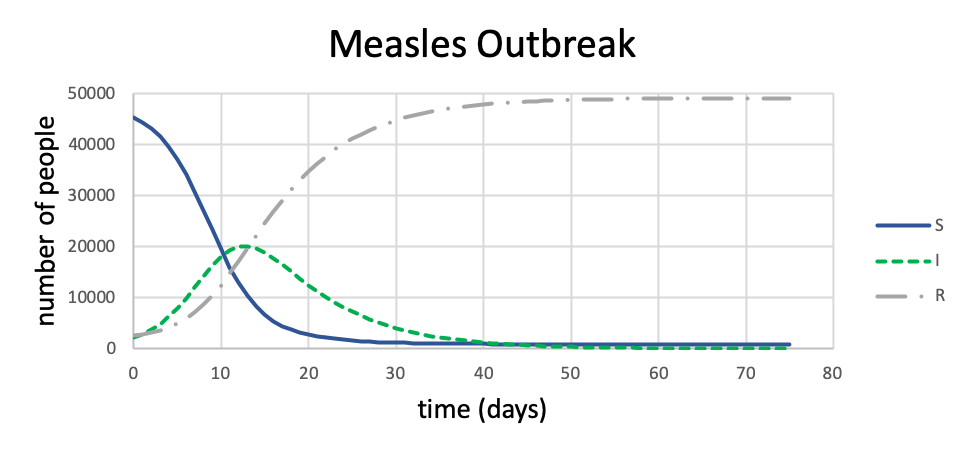
\includegraphics[scale = 0.75]{measles_plot.png}
	\end{center}

\noindent  At this point, let's take a moment to reflect on what we did.  We came up with a mathematical 
model for the outbreak of a disease.  While we could not come up with an analytical solution (i.e., we
can't write a formula for $S(t),$  $I(t)$, or $R(t)$), we were able to come up with a {numerical solution}
for the system of DEs.  That is, we can give the approximate value of the $S(t),$ $I(t)$, and $R(t)$ at
specific $t$-values.  We don't have formulas, but we can ``see'' loads of information about how we
believe the outbreak might progress.\\

\noindent  Before we began, we made a guess about how we thought the populations would change
over time.  If we look back at those plots, we see that the actual solution we generated is just like those.
In other words, our model behaves just how we think it should.\\

\end{document}
